\section{Results}
\label{sec:results}
The pilot used 480 images and training seeds 42, 43 and 44. Both detectors had lower F1 on Midjourney than on familiar generators. The original unseen CLIP-minus-ResNet difference reached the prespecified statistical significance level, while CLIP exceeded the false-positive target. Neither model met all project success criteria. RQ1 concerns unseen-generator detection and false positives on real images. RQ2 concerns the changes after JPEG compression and resizing. The matched 20,000-image study remains planned.

\subsection{Data actually used and departures from the full study}
\label{sec:results-data}
We accessed the Tiny-GenImage mirror \citep{tinygen2026} on 17 October 2026 and recorded revision \texttt{89c4fe9efd0e}. The sampling frame contained the first 1,200 training and 600 validation metadata rows. Sampling seed 42 selected 480 images. The remaining 1,320 rows were outside the sample and were not cleaning removals. All selected assets downloaded and decoded successfully. SHA256 checks found no exact duplicate group. The same manifest and image hashes were used for each training seed; none of the additional runs selected new images.

Training contained 120 real images, 60 BigGAN images and 60 GLIDE images. Validation contained 40 real images and 20 from each development generator. The seen test used the same source counts as validation with different IDs. The unseen test contained 40 real images and 40 Midjourney images. Midjourney was absent from training and validation. Table~\ref{tab:dataset} records these pilot counts beside the full-study targets. The reserved tests contain 160 distinct images, each evaluated in three conditions by two models across three runs.

\begin{table}[!htbp]
\caption{Preliminary sample actually used. Full-study targets are shown separately. All pilot rows were readable; no exact duplicate group was found among the 480 selected files. Source: Tiny-GenImage mirror, accessed 17 October 2026.}
\label{tab:dataset}
\centering
\small
\setlength{\tabcolsep}{3.5pt}\renewcommand{\arraystretch}{1.15}
\begin{tabularx}{\linewidth}{@{}Yrrrr@{}}
\toprule
Partition & Full target & Pilot $n$ & Real & Generated\\
\midrule
Training & 12,000 & 240 & 120 & 120\\
Validation & 2,000 & 80 & 40 & 40\\
Seen test & 2,000 & 80 & 40 & 40\\
Unseen test & 4,000 & 80 & 40 & 40\\
Total & 20,000 & 480 & 240 & 240\\
\bottomrule
\end{tabularx}
\end{table}


The pilot used the public mirror, omitted SD 1.4 from development and retained the small sample before matching. Perceptual duplicate screening, category matching and matching of native size and JPEG tables were not completed. These departures from the full design are recorded with the manifest. The training-seed repeats changed model initialization and training order while preserving image IDs, source labels and split assignments. Repeated scores for an image therefore remain observations on that same image.

All retrieved assets decoded as JPEG. Real-image widths ranged from 139 to 2,048 pixels and heights from 127 to 1,536. BigGAN images were $128\times128$, GLIDE images $256\times256$ and Midjourney images $1024\times1024$. Original compression histories and category balance remain unresolved. These measurements describe the mirror assets. The official archives still require inspection before confirming the 20,000-image target and the counts retained after cleaning and matching. No official-archive audit count is reported as an observed pilot total.
\FloatBarrier

\subsection{RQ1 original-image detection and transfer}
\label{sec:results-rq1}
Table~\ref{tab:main-results} reports mean run-level metrics with sample standard deviations at threshold 0.5. On familiar generators, ResNet-50 achieved mean F1 0.972 (SD 0.018), compared with 0.870 (SD 0.017) for CLIP linear. Mean FPR was 0.058 (SD 0.038) for ResNet and 0.267 (SD 0.029) for CLIP. ResNet detected all 40 generated images in every run. CLIP detected 40, 39 and 38 for seeds 42, 43 and 44, respectively.

\begin{table}[!htbp]
\caption{Original-image metrics at threshold 0.5. Upper cells show mean with sample SD in parentheses over training seeds 42, 43 and 44; lower rows show unseen confusion counts for each run. Each test has 40 real and 40 generated images, reused across seeds. P and R are precision and recall; AUC is AUROC.}
\label{tab:main-results}
\centering
\fontsize{8.5}{10.5}\selectfont
\setlength{\tabcolsep}{3.2pt}\renewcommand{\arraystretch}{1.10}
\begin{tabularx}{\linewidth}{@{}llCCCCCCC@{}}
\toprule
Model & Test & Acc. & P & R & F1 & FPR & AUC & AP\\
\midrule
ResNet-50 & Seen & \shortstack{0.971\\{(0.019)}} & \shortstack{0.946\\{(0.034)}} & \shortstack{1.000\\{(0.000)}} & \shortstack{0.972\\{(0.018)}} & \shortstack{0.058\\{(0.038)}} & \shortstack{0.999\\{(0.002)}} & \shortstack{0.999\\{(0.002)}}\\
CLIP linear & Seen & \shortstack{0.854\\{(0.019)}} & \shortstack{0.785\\{(0.018)}} & \shortstack{0.975\\{(0.025)}} & \shortstack{0.870\\{(0.017)}} & \shortstack{0.267\\{(0.029)}} & \shortstack{0.946\\{(0.005)}} & \shortstack{0.946\\{(0.005)}}\\
ResNet-50 & Unseen & \shortstack{0.504\\{(0.014)}} & \shortstack{0.556\\{(0.509)}} & \shortstack{0.025\\{(0.025)}} & \shortstack{0.047\\{(0.047)}} & \shortstack{0.017\\{(0.014)}} & \shortstack{0.487\\{(0.088)}} & \shortstack{0.527\\{(0.061)}}\\
CLIP linear & Unseen & \shortstack{0.458\\{(0.014)}} & \shortstack{0.392\\{(0.046)}} & \shortstack{0.158\\{(0.038)}} & \shortstack{0.225\\{(0.046)}} & \shortstack{0.242\\{(0.014)}} & \shortstack{0.518\\{(0.010)}} & \shortstack{0.519\\{(0.011)}}\\
\bottomrule
\end{tabularx}
\medskip
\begin{tabularx}{\linewidth}{@{}Yrrrrr@{}}
\toprule
Unseen counts: model & Seed & TP & FP & TN & FN\\
\midrule
ResNet-50 & 42 & 2 & 1 & 39 & 38\\
ResNet-50 & 43 & 0 & 1 & 39 & 40\\
ResNet-50 & 44 & 1 & 0 & 40 & 39\\
CLIP linear & 42 & 8 & 10 & 30 & 32\\
CLIP linear & 43 & 6 & 10 & 30 & 34\\
CLIP linear & 44 & 5 & 9 & 31 & 35\\
\bottomrule
\end{tabularx}
\end{table}


On the original unseen set, mean ResNet F1 was 0.047 (SD 0.047), with mean recall 0.025 and mean FPR 0.017. Its true-positive counts were two, zero and one. CLIP's mean F1 was 0.225 (SD 0.046), recall was 0.158 and FPR was 0.242. Its true-positive counts were eight, six and five. The lower part of Table~\ref{tab:main-results} gives TP, FP, TN and FN separately for each unseen run. Every count row covers the same 40 real and 40 generated images.

The original unseen mean AUROC was 0.487 (SD 0.088) for ResNet and 0.518 (SD 0.010) for CLIP. Their mean AP values were 0.527 and 0.519. Mean accuracy was 0.504 for ResNet and 0.458 for CLIP. On familiar images, mean AUROC and AP rounded to 0.999 for ResNet and 0.946 for CLIP. Table~\ref{tab:main-results} also includes precision and recall, averaged after calculation for each run.

The mean seen-to-unseen F1 drops were 0.925 for ResNet and 0.645 for CLIP, exceeding the 0.10 limit. Both mean unseen F1 values were below 0.80. ResNet's FPR stayed within 0.10 on both original tests in all three runs. CLIP exceeded that limit on both tests in each run. Neither detector satisfied all project goals in any run: the count was zero of three for each baseline. These checks use the fixed primary threshold and original-image conditions.

Seen false-positive counts for ResNet were four, one and two in seed order; CLIP's were ten, twelve and ten. Individual seen F1 ranged from 0.952 to 0.988 for ResNet and 0.857 to 0.889 for CLIP. Original unseen F1 ranged from 0.000 to 0.093 and from 0.185 to 0.276, respectively. ResNet seed 43 produced no correct generated-class detection on the original unseen set. Its unseen false-positive count was one.
\FloatBarrier

\subsection{Paired uncertainty and statistical testing}
\label{sec:results-uncertainty}
The primary difference in mean original unseen F1, CLIP minus ResNet, was 0.178. Its paired bootstrap 95\% interval was [0.052, 0.316], with permutation p-value 0.0261 (Table~\ref{tab:paired}). The interval excluded zero and the p-value was below 0.05. CLIP's mean unseen FPR of 0.242 exceeded the practical target of 0.10. The observed F1 gap therefore passed the statistical test and the minimum-gap requirement, but failed the FPR requirement for a practically meaningful advantage.

\begin{table}[!htbp]
\caption{Mean F1 differences (CLIP minus ResNet), with paired 95\% intervals. The original-unseen test is the main exploratory comparison; secondary p-values are unadjusted.}
\label{tab:paired}
\centering
\small
\setlength{\tabcolsep}{3.2pt}\renewcommand{\arraystretch}{1.10}
\begin{tabularx}{\linewidth}{@{}lYccc@{}}
\toprule
Test & Condition & $\Delta F_1$ & 95\% CI & $p$\\
\midrule
Seen & Original & -0.071 & [-0.090, -0.053] & 0.0001\\
Seen & JPEG 65 & -0.067 & [-0.088, -0.048] & 0.0001\\
Seen & Resize 112 & -0.028 & [-0.033, -0.021] & 0.0001\\
Unseen & Original & 0.483 & [0.437, 0.527] & 0.0001\\
Unseen & JPEG 65 & 0.458 & [0.409, 0.505] & 0.0001\\
Unseen & Resize 112 & 0.006 & [-0.004, 0.016] & 0.2829\\
\bottomrule
\end{tabularx}
\end{table}


On familiar original images, the CLIP-minus-ResNet difference was $-0.102$, with interval [$-0.159$, $-0.047$] and p-value 0.0004. The corresponding JPEG-compressed seen difference was $-0.121$, with p-value 0.0003. These are secondary comparisons. The original unseen comparison remains primary; the other p-values are descriptive and have no multiple-comparison adjustment. Table~\ref{tab:paired} retains the sign of the difference for every condition. ResNet's original unseen AUROC values were 0.409, 0.471 and 0.582 across seeds. CLIP's were 0.524, 0.523 and 0.506. ResNet precision on that set ranged from 0.000 to 1.000, with mean 0.556 and SD 0.509.

For JPEG-compressed unseen images, the mean difference was 0.171, with interval [0.043, 0.308] and p-value 0.0405. For resized unseen images, it was 0.012, with interval [$-0.018$, 0.044] and p-value 0.4139. The resized difference was below the 0.03 practical minimum. On familiar resized images, the difference was $-0.027$, also below that minimum, with p-value 0.0016. None of these processing comparisons met all the declared practical criteria.

The three completed runs permit sample standard deviations over training runs. The image-bootstrap intervals remain conditional on the three fitted checkpoint pairs, using the paired procedures in Section~\ref{sec:methods}. Each test still has only 40 real images, so one changed decision changes a single run's FPR by 0.025. The three training seeds reuse those images. Individual confusion counts, across-run SDs and image-sampling intervals are reported separately, with no increase in the stated number of independent test images.
\FloatBarrier

\subsection{RQ2 processing changes}
\label{sec:results-rq2}
All reserved test images produced both processed versions successfully. No image was excluded from a paired comparison. Table~\ref{tab:robustness} gives mean processed-minus-original changes and paired 95\% intervals for both F1 and FPR. Figure~\ref{fig:conditions} gives absolute unseen scores averaged over the three runs, with image-bootstrap intervals. The full-study reference levels remain F1 at least 0.80 and FPR at most 0.10. The processing conditions use separate transformations of the same originals.

\begin{table}[!htbp]
\caption{Preliminary robustness changes, processed minus original. Negative $\Delta F_1$ and positive $\Delta\mathrm{FPR}$ indicate deterioration. All comparisons contain the same 80 image IDs per test. Full paired intervals are in the evaluation export; values use score units on a 0--1 scale.}
\label{tab:robustness}
\centering
\small
\setlength{\tabcolsep}{3.5pt}\renewcommand{\arraystretch}{1.15}
\begin{tabularx}{\linewidth}{@{}llCCCC@{}}
\toprule
Model & Test & JPEG $\Delta F_1$ & JPEG $\Delta$FPR & 112 $\Delta F_1$ & 112 $\Delta$FPR\\
\midrule
ResNet-50 & Seen & 0.012 & -0.025 & -0.292 & 0.900\\
CLIP linear & Seen & -0.012 & 0.000 & -0.222 & 0.750\\
ResNet-50 & Unseen & 0.000 & 0.000 & 0.560 & 1.000\\
CLIP linear & Unseen & -0.058 & -0.025 & 0.391 & 0.750\\
\bottomrule
\end{tabularx}
\end{table}


\begin{figure}[!htbp]
\centering
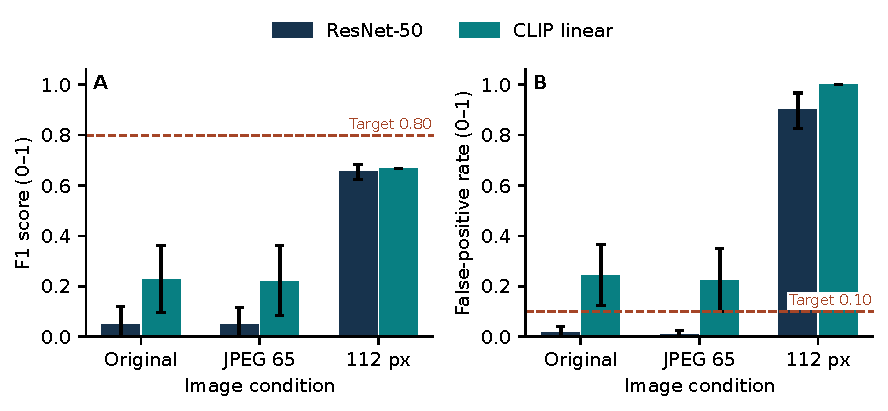
\includegraphics[width=\linewidth]{figures/pilot_condition_comparison.pdf}
\caption{Mean unseen performance over training seeds 42, 43 and 44 on 80 distinct images. Error bars are paired image-bootstrap 95\% intervals conditional on the fitted models. Scores use a 0--1 scale. Dashed lines mark the full-study F1 minimum 0.80 and FPR maximum 0.10.}
\label{fig:conditions}
\end{figure}

After JPEG quality 65, ResNet's mean unseen F1 stayed at 0.047. The paired F1 change was zero in every run, giving interval [0.000, 0.000]. Its FPR change was $-0.008$, with interval [$-0.025$, 0.000]. CLIP's mean unseen F1 was 0.218, a change of $-0.007$ with interval [$-0.074$, 0.069]. Its FPR change was $-0.017$, with interval [$-0.075$, 0.025]. The corresponding absolute mean FPRs were 0.008 for ResNet and 0.225 for CLIP.

Downsampling increased mean unseen ResNet F1 by 0.608, with interval [0.534, 0.667], to 0.655. CLIP F1 increased by 0.442, with interval [0.314, 0.568], to 0.667. Mean FPR increased by 0.883 for ResNet and 0.758 for CLIP, reaching 0.900 and 1.000. CLIP labelled all 40 real images generated in each resized unseen run. Both models exceeded the false-positive target after this transformation.

On familiar generators, JPEG changed mean F1 by 0.008 for ResNet and $-0.011$ for CLIP; both intervals crossed zero. Their FPR changes were $-0.025$ and 0.008. Resizing reduced mean F1 by 0.278 and 0.203, with intervals [$-0.306$, $-0.245$] and [$-0.260$, $-0.150$]. Mean FPR rose by 0.825 and 0.733. All main processing intervals are shown in Table~\ref{tab:robustness}. The experiment covered JPEG quality 65 and downsampling to 112 pixels; no wider JPEG-quality sweep was run.
\FloatBarrier

\subsection{Sensitivity to the decision threshold}
\label{sec:results-sensitivity}
The validation rule selected ResNet thresholds 0.85, 0.60 and 0.30 for seeds 42, 43 and 44. It selected 0.50 for CLIP in every run. These choices used validation predictions only. Table~\ref{tab:sensitivity} compares them with the primary threshold 0.50 on identical original test IDs. It lists each threshold and the mean test scores with sample SDs. The underlying model checkpoints and continuous scores were fixed during this comparison.

\begin{table}[!htbp]
\caption{Original-image threshold sensitivity. Thresholds are listed for seeds 42, 43 and 44, in that order. F1 and FPR averages and sample SDs occupy separate columns. Each validation threshold is selected independently using only validation predictions. Each run evaluates the same 80 images per test.}
\label{tab:sensitivity}
\centering
\fontsize{8.5}{10.5}\selectfont
\setlength{\tabcolsep}{3.2pt}\renewcommand{\arraystretch}{1.10}
\begin{tabularx}{\linewidth}{@{}llYccccc@{}}
\toprule
Model & Test & Rule & $t_{42},t_{43},t_{44}$ & F1 & SD & FPR & SD\\
\midrule
ResNet-50 & Seen & Fixed & 0.50, 0.50, 0.50 & 0.972 & 0.018 & 0.058 & 0.038\\
ResNet-50 & Seen & Validation & 0.85, 0.60, 0.30 & 0.980 & 0.007 & 0.042 & 0.014\\
ResNet-50 & Unseen & Fixed & 0.50, 0.50, 0.50 & 0.047 & 0.047 & 0.017 & 0.014\\
ResNet-50 & Unseen & Validation & 0.85, 0.60, 0.30 & 0.033 & 0.028 & 0.000 & 0.000\\
CLIP linear & Seen & Fixed & 0.50, 0.50, 0.50 & 0.870 & 0.017 & 0.267 & 0.029\\
CLIP linear & Seen & Validation & 0.50, 0.50, 0.50 & 0.870 & 0.017 & 0.267 & 0.029\\
CLIP linear & Unseen & Fixed & 0.50, 0.50, 0.50 & 0.225 & 0.046 & 0.242 & 0.014\\
CLIP linear & Unseen & Validation & 0.50, 0.50, 0.50 & 0.225 & 0.046 & 0.242 & 0.014\\
\bottomrule
\end{tabularx}
\end{table}


At its validation-selected thresholds, ResNet's mean seen F1 was 0.980 and mean FPR was 0.042. At 0.50 they were 0.972 and 0.058. For seed 42, the selected threshold reduced seen false positives from four to two. Seeds 43 and 44 retained their seen decisions. Each ResNet run still detected all 40 familiar generated images. The threshold choices therefore changed the reported seen averages through seed 42's real-image decisions.

On Midjourney, ResNet's validation-selected mean F1 was 0.033 and mean FPR was zero. The true-positive counts were one, zero and one. At threshold 0.50 those counts had been two, zero and one. CLIP's seen and unseen metrics were unchanged in every run because all its selected thresholds equalled 0.50. AUROC and AP were unchanged for both models throughout the threshold comparison. There was no retraining in this analysis.

Validation contained 80 images from the development sources. The selected thresholds apply to this pilot's validation samples, with the same image IDs across runs. The future matched-data experiment will select its own thresholds under the declared rule. The fixed 0.50 results remain primary, and no threshold was chosen from unseen test performance. The sensitivity export contains individual-run scores as well as the averages in Table~\ref{tab:sensitivity}.
\FloatBarrier

\subsection{Observed errors}
\label{sec:results-errors}
Across original unseen runs, ResNet missed 38, 40 and 39 Midjourney images. CLIP missed 32, 34 and 35. ResNet incorrectly flagged one, one and zero real images; CLIP flagged ten, ten and nine. Figure~\ref{fig:errors} shows the confusion matrices and inspected error examples for seed 42. That run made 39 unseen errors with ResNet and 42 with CLIP. The full three-run unseen counts remain in Table~\ref{tab:main-results}.

\begin{figure}[!htbp]
\centering
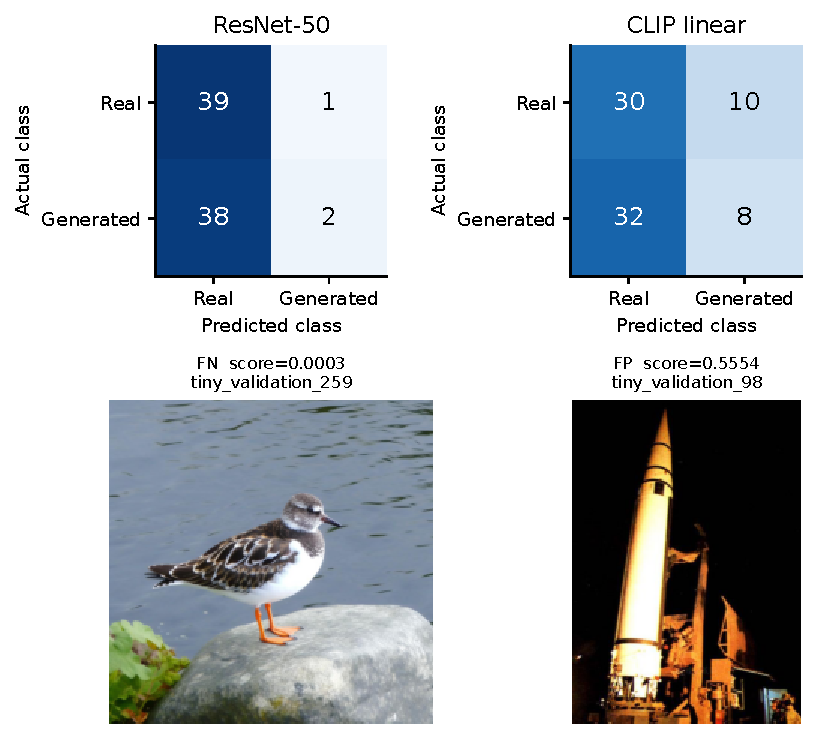
\includegraphics[width=0.90\linewidth]{figures/pilot_errors.pdf}
\caption{Illustrative original-unseen errors for seed 42 only, threshold 0.5; all three runs are counted in Table~\ref{tab:main-results}. Matrix cells count images, with actual class on rows and predicted class on columns. Lower panels show the most confident ResNet false negative and CLIP false positive within those error types. Scores are generated-class sigmoid outputs. Images and labels are from Tiny-GenImage \citep{tinygen2026}; IDs identify manifest records.}
\label{fig:errors}
\end{figure}

On seen BigGAN images ($128\times128$ pixels), mean recall was 1.000 for both models. On GLIDE ($256\times256$), it was 1.000 for ResNet and 0.950 (SD 0.050) for CLIP. On held-out Midjourney ($1024\times1024$), mean recalls were 0.025 and 0.158. Each seen generator contributed 20 images per test run. Native-size and content-category effects remain unseparated in this pilot. Dimensions, source groups and individual error records are retained for later grouped checks.

The selected ResNet miss was a Midjourney-labelled bird image with generated-class score 0.000287. The selected CLIP false positive was a real-labelled image with score 0.555357. Both examples came from seed 42's original unseen predictions. The examples use dataset labels to define errors. For each indicated error type, selection used the largest score distance from 0.5. The complete export retains IDs, scores, conditions, seeds and error types for all model errors. We kept checkpoints and training settings fixed after inspection. The recorded findings include low original unseen detection, zero ResNet JPEG F1 change, unchanged CLIP threshold choices and high FPR after resizing.
\FloatBarrier

\subsection{Observed setup and reproducibility}
\label{sec:results-reproducibility}
All three reported runs used the AMD CPU setup in Table~\ref{tab:reproducibility}. ResNet completed one epoch per run, with training losses from 0.324 to 0.399 and validation F1 from 0.949 to 1.000. Each CLIP head completed 40 epochs. Its final-epoch training losses ranged from 0.528 to 0.531. The selected head checkpoints were epochs 40, 21 and 34 for seeds 42, 43 and 44, with validation F1 values 0.964, 0.952 and 0.976.

\begin{table}[!htbp]
\caption{Observed preliminary-run setup. Training times include tensor preparation and, for CLIP, development feature extraction. Prediction times are warmed model-only medians for one image. No GPU was used.}
\label{tab:reproducibility}
\centering
\small
\setlength{\tabcolsep}{3.5pt}\renewcommand{\arraystretch}{1.15}
\begin{tabularx}{\linewidth}{@{}lY@{}}
\toprule
Item & Observed setting\\
\midrule
Source and revision & \texttt{TheKernel01/Tiny-GenImage}, revision \texttt{89c4fe9efd0e}\\
Device & Intel Xeon Platinum 8573C; six PyTorch threads; 8 GiB container\\
Python and core libraries & 3.12.14; PyTorch 2.14.1+cpu; torchvision 0.29.1+cpu\\
Other libraries & CLIP 1.0.1; NumPy 2.5.2; Pillow 12.3.0; scikit-learn 1.8.0; SciPy 1.17.0\\
Seed and optimizers & Global seed 42; Adam; learning rates $10^{-4}$ (ResNet), $10^{-3}$ (head)\\
Epochs and batch sizes & ResNet: 1 epoch, batch 8; CLIP head: 40 epochs, batch 32\\
Preparation and training & ResNet 43.76 s; CLIP 30.50 s\\
Prediction median & ResNet 63.01 ms/image; CLIP 158.09 ms/image\\
End-to-end pilot & 386.06 s including data access and model loading\\
Repository & \url{https://github.com/C0nflu3nc3/RMT}; scripts, manifest, predictions, versions and training logs\\
\bottomrule
\end{tabularx}
\end{table}


Per-run elapsed times were 130.93, 94.17 and 151.10 seconds. These runs reused the hash-verified image cache. Mean preparation/training times were 41.79 seconds for ResNet and 11.21 for CLIP, including development feature extraction for CLIP. Warmed single-image prediction medians ranged from 36.43 to 46.29 milliseconds for ResNet and 45.91 to 370.78 for CLIP. The measurements came from a shared CPU host. Software installation and subsequent statistical analysis were outside the elapsed totals.

The archive contains all 2,880 test prediction rows, validation scores, the 480-image manifest and per-run histories. The score-only reproduction command rebuilds Tables 2--5 in an isolated copy and checks them against the supplied LaTeX tables. It requires no GitHub connection, image download, model weights or PyTorch. The repository is private; the ZIP includes the required scripts and score files. The earlier Intel feasibility run is retained separately and excluded from the three-run aggregates. Official-archive auditing and the matched-data experiment remain future work.
\FloatBarrier
